\section*{8.11}

The source code is presented as \href{run:./8_11.cpp}{8\_11.cpp}.

To transpose a matrix, we first gather the matrix to a single processor, then scatter the matrix to all processors. 

For processors other than the root processor, they send the data to the root processor, and then receive the data from the root processor.

\begin{lstlisting}[language=C++]
    MPI_Gatherv(buffer, buffer_size, MPI_INT, NULL, 
        NULL, NULL, MPI_INT, 0, MPI_COMM_WORLD);
    MPI_Scatterv(NULL, NULL, NULL, MPI_INT, buffer, 
        buffer_size, MPI_INT, 0, MPI_COMM_WORLD);
\end{lstlisting}

For the root processor, it need to calculate the displacement and block size for each processor, and then gather the data from all processors and scatter the data to all processors.

\begin{lstlisting}[language=C++]
    int *matrix_buffer = new int[N * N];
    int *displs = new int[p];
    int *receive_counts = new int[p];
    for (int i = 0; i < p; i++) {
        displs[i] = BLOCK_LOW(i, p, N) * N;
        receive_counts[i] = BLOCK_SIZE(i, p, N) * N;
    }
    MPI_Gatherv(buffer, buffer_size, MPI_INT, matrix_buffer, 
        receive_counts, displs, MPI_INT, 0, MPI_COMM_WORLD);
    for (int i = 0; i < N; i++) {
        for (int j = i + 1; j < N; j++) {
            int temp = matrix_buffer[i * N + j];
            matrix_buffer[i * N + j] = matrix_buffer[j * N + i];
            matrix_buffer[j * N + i] = temp;
        }
    }
    MPI_Scatterv(matrix_buffer, receive_counts, displs, MPI_INT, 
        buffer, buffer_size, MPI_INT, 0, MPI_COMM_WORLD);
    delete[] matrix_buffer;
    delete[] displs;
    delete[] receive_counts;
\end{lstlisting}

The snapshot of the result is shown in Figure \ref{fig:8_11}. As we can see, the matrix is transposed correctly.

\begin{figure}[H]
    \centering
    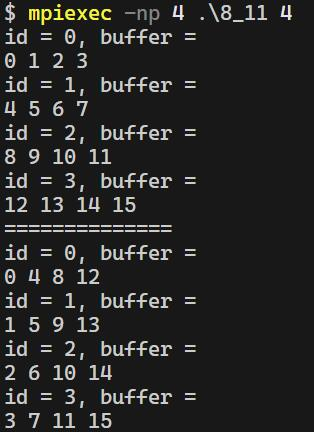
\includegraphics[width=0.2\textwidth]{fig-8_11.jpg}
    \caption{Snapshot of the result of 8.11}
    \label{fig:8_11}
\end{figure}

\section*{9.8}

The source code is presented as \href{run:./9_8.cpp}{9\_8.cpp}.

For each worker, it will receive $x$ from the manager, calculate $f(x)$, and send the result $x,y$ back to the manager.

\begin{lstlisting}[language=C++]
void worker()
{
    double buffer[2];
    while(true)
    {
        MPI_Recv(&buffer, 1, MPI_DOUBLE, 0, 0, 
            MPI_COMM_WORLD, MPI_STATUS_IGNORE);
        if (buffer[0] < 0) break;
        buffer[1] = f(buffer[0]);
        MPI_Send(&buffer, 2, MPI_DOUBLE, 0, 0, MPI_COMM_WORLD);
    }
}
\end{lstlisting}

For the manager, it will split the interval $[a,b]$ into $p$ subintervals, and send these $p-1$ split points to the workers. Then, it will receive the results from the workers and check for the new interval.

\begin{lstlisting}[language=C++]
void manager(int p)
{
    double low = 0.0;
    double high = 1.0;
    while (high - low > 1e-11)
    {
        double interval = (high - low) / p;
        for (int i = 1; i < p; ++i)
        {
            double x = low + i * interval;
            MPI_Send(&x, 1, MPI_DOUBLE, i, 0, MPI_COMM_WORLD);
        }
        for (int i = 1; i < p; ++i)
        {
            double buffer[2];
            MPI_Recv(&buffer, 2, MPI_DOUBLE, i, 0,
                MPI_COMM_WORLD, MPI_STATUS_IGNORE);
            if (buffer[1] > 0) high = MIN(high, buffer[0]);
            else low = MAX(low, buffer[0]);
        }
    }
    // terminate workers
    for (int i = 1; i < p; ++i)
    {
        double x = -1;
        MPI_Send(&x, 1, MPI_DOUBLE, i, 0, MPI_COMM_WORLD);
    }
    printf("The root is %.10f\n", (low + high) / 2);
}
\end{lstlisting}

The snapshot of the result is shown in Figure \ref{fig:9_8}.

\begin{figure}[H]
    \centering
    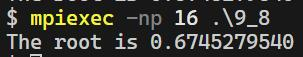
\includegraphics[width=0.3\textwidth]{fig-9_8.jpg}
    \caption{Snapshot of the result of 9.8}
    \label{fig:9_8}
\end{figure}

\section*{11.4}
(1)
The computational time of each iteration is
$$
\chi\frac{n}{p}\frac{n}{p}n=\chi\frac{n^3}{p^2}
$$

The communication time of each iteration is
$$
\lambda + \frac{n\frac{n}{p}}{\beta} = \lambda + \frac{n^2}{p\beta}
$$

When the communication time is less than the computational time, we have
$$
\lambda + \frac{n^2}{p\beta} < \chi\frac{n^3}{p^2}
$$
the solution is $n>1072.2$, so $n$ should be at least 1073.

(2)
The computational time of each iteration is
$$
\chi\frac{n}{\sqrt p}^3=\chi\frac{n^3}{p^{3/2}}
$$

The communication time of each iteration is
$$
2\left(\lambda + \frac{\frac{n}{\sqrt p}^2}{\beta}\right) = 2\lambda + \frac{2n^2}{p\beta}
$$

When the communication time is less than the computational time, we have

$$
2\lambda + \frac{2n^2}{p\beta} < \chi\frac{n^3}{p^{3/2}}
$$
the solution is $n>544.1$, so $n$ should be at least 545.

\section*{14.9}

(a)

The algorithm is presented as Algorithm \ref{alg:parallel-merge-sort}. We split the data into $p$ partitions, and each processor sorts its own partition. Then, we merge the partitions in a binary tree fashion. The communication flow is shown in Figure \ref{fig:communication-flow}.

\begin{algorithm}
    \SetAlgoLined
    \caption{Parallel Merge Sort}
    \label{alg:parallel-merge-sort}
    \BlankLine
    \KwIn{Number of processors $p$, Rank of current processor $rank$}
    \KwOut{Sorted array $A$}
    \BlankLine
    Receive own partition of data $A$\;
    $\textsc{Sort}(A)$\;
    $s \leftarrow 1$\;
    \While{$2^s\leq p$}{
        \uIf{$rank \mod 2^s = 0$}{
            Receive $B$ from $rank+2^{s-1}$\;
            $A \leftarrow \textsc{Merge}(A, B)$\;
            $s \leftarrow s+1$\;
        }
        \Else{
            Send $A$ to $rank-2^{s-1}$\;
            Break\;
        }
    }
    \If{$rank = 0$}{
        \Return{$A$}\;
    }
\end{algorithm}

\begin{figure}
    \centering
    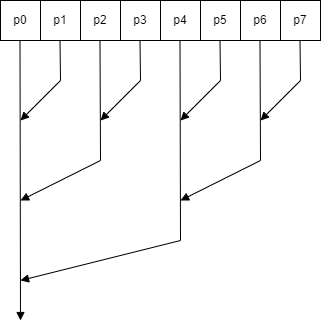
\includegraphics[width=0.5\textwidth]{fig-dataflow.png}
    \caption{Communication flow of parallel merge sort}
    \label{fig:communication-flow}
\end{figure}

\noindent(b)

Firstly, every processor needs to merge its own partition locally, the time complexity to sort $n/p$ elements is $\Theta((n/p)\log(n/p))$. The total time complexity is $\Theta(n\log(n/p))$.

Then, denote $p=2^k$, $k$ merge is needed. For the $i$-th merge, there are $2^{k-i}$ working processors and each merges $\frac{2^in}{p}$ elements. So the time complexity of inter-processor merging stage is
\begin{align*}
    \sum_{i=1}^k 2^{k-i}\Theta\left(\frac{2^in}{p}\right) &= \Theta\left(\sum_{i=1}^k n\right)\\
    &= \Theta\left(nk \right)\\
    &= \Theta(n\log p)
\end{align*}

The time complexity of this algorithm is $\Theta(n\log p)+\Theta(n\log(n/p))=\Theta(n\log n)$.

\noindent(c)

If we only use one processor, the time complexity is $\Theta(n\log n)$.

If we use $p$ processors, the processor $0$ will do the most work, and the other processors will do less work. The computation time of processor $0$ is $\Theta\left(\frac{n}{p}\log\frac{n}{p}+\sum_{i=1}^{\log p}\frac{2^in}{p}\right)=\Theta\left(\frac{n}{p}\log\frac{n}{p}+n\right)$. The communication time of processor $0$ is $\Theta\left(\sum_{i=1}^{\log p}\frac{2^{i-1}n}{p}\right)=\Theta(n)$. 

Thus, $T(n,1)=\Theta(n\log n)$, $T(n,p)=\Theta\left(\frac{n}{p}\log\frac{n}{p}+n\right)$, and $T_0(n,p)=p\Theta\left(\frac{n}{p}\log\frac{n}{p}+n\right)-\Theta(n\log n)=\Theta(np-n\log p)$. 

So, the isoefficiency function is given by
$$
n\log n \geq C(np-n\log p)\\
\Rightarrow n \geq \frac{e^{pC}}{p^C}
$$

\noindent(d)

The source code is presented as \href{run:./14_9.cpp}{14\_9.cpp}.

In each iteration, if the processor already fininshed all its work, it will send its sorted subarray to another processor and break the loop.

\begin{lstlisting}[language=C++]
    int target_id = id >> aggregate_size << aggregate_size;
    MPI_Send(&local_buffer_size, 1, MPI_INT, target_id, 0, MPI_COMM_WORLD);
    MPI_Send(sorted_buffer, local_buffer_size, 
        MPI_INT, target_id, 0, MPI_COMM_WORLD);
    delete[] sorted_buffer;
    break;
\end{lstlisting}

Otherwise, a processor will receive the sorted subarray from another processor and merge them.

\begin{lstlisting}[language=C++]
    int *local_part = sorted_buffer;
    sorted_buffer = NULL;
    int source_id = id + (0x1 << (aggregate_size - 1));
    int receive_buffer_size;
    MPI_Recv(&receive_buffer_size, 1, MPI_INT, source_id, 
        0, MPI_COMM_WORLD, MPI_STATUS_IGNORE);
    receive_buffer = new int[receive_buffer_size];
    MPI_Recv(receive_buffer, receive_buffer_size, MPI_INT, 
        source_id, 0, MPI_COMM_WORLD, MPI_STATUS_IGNORE);
    sorted_buffer = new int[local_buffer_size + receive_buffer_size];
    merge(local_part, local_buffer_size, receive_buffer, 
        receive_buffer_size, sorted_buffer);
    delete[] local_part;
    delete[] receive_buffer;
    local_buffer_size += receive_buffer_size;
    aggregate_size++;
\end{lstlisting}

The benchmark results are shown in Table \ref{tab:benchmark}. As we can see, for a small number of elements, the communication time is much larger than the computation time, so the parallel version is slower than the serial version. However, as the number of elements increases, the parallel version becomes faster than the serial version.

\begin{table}[H]
    \centering
    \caption{Benchmark results for various combinations of p and n (in seconds)}
    \label{tab:benchmark}
    \begin{tabular}{c|cccc}
    \hline
    \diagbox{n}{p}  & 1        & 2        & 4        & 8        \\ \hline
    100       & 0.000022 & 0.000100 & 0.000385 & 0.001196 \\
    10,000    & 0.001697 & 0.000865 & 0.001110 & 0.001705 \\
    1,000,000 & 0.186246 & 0.105908 & 0.058725 & 0.045571 \\ \hline
    \end{tabular}
\end{table}